\RequirePackage{fixltx2e}
\documentclass{jknotes}
\usepackage{joshkirklin}

\begin{document}

\institution{Cambridge Part III Maths}
\title{Applications of Differential Geometry to Physics}
\lecturer{Maciej Dunajski}
\notetaker{Josh Kirklin}
\date{Lent 2016}

\maketitle
\suggestionsspiel
\tableofcontents

\section{Introduction}
\lecture{14/01/16}
Geometry has always played a key role in physics. For example, consider Kepler orbits, i.e. paths \(\vb{r}(t)\) in \(\RR^3\) obeying:
\begin{equation}
    \dot{\vb{r}} = \frac{GM}{r^3}\vb{r}
\end{equation}

\begin{wrapfigure}{l}{0.3\linewidth}
    \centering
    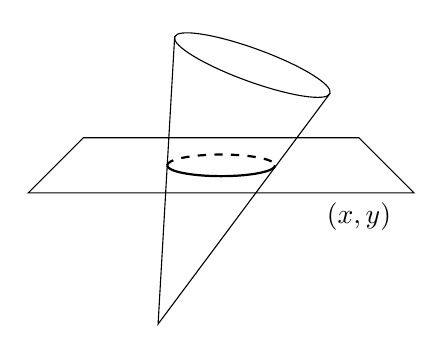
\begin{tikzpicture}[scale=0.7]
        \node[below] at (6,0) {\((x,y)\)};
        \draw (0,0) -- (1,1) -- (6,1) -- (7,0) -- cycle;
        \begin{scope}[shift={(3.5,0.5)},yscale=0.2,thick]
            \draw (-0.98,0) arc (-180:0:0.98);
            \draw[dashed] (-0.98,0) arc (180:0:0.98);
        \end{scope}
        \begin{scope}[shift={(3.04,-0.5)}, rotate=-20]
            \draw (-1.5,3) -- (0,-2) -- (1.5,3);
            \draw (0,3) ellipse (1.5 and 0.3);
        \end{scope}
    \end{tikzpicture}
\end{wrapfigure}
The solutions are conic sections. If we view a conic section as a path with coordinates \((x,y)\) in the plane it inhabits, then we can find that all conic sections can be written as the locus of solutions of an equation of the following form:
\begin{equation}
    ay^2 +  bx^2 + cxy + dy + ex + f = 0
\end{equation}
where \(a,b,c,d,e,f \in\RR\). It was first deduced by Apollonius of Perga that given five arbitrary points in the plane, there is a unique conic section through those points. Thus if we observe the position of a planet at five different points, we can deduce its orbit.

The space of conic sections is \(\mathbb{RP}^5=\RR^6/\sim\) where \(x\sim y \iff \Exists C \in \RR \st x = Cy\). We can see this by first labelling each conic section by its coefficients \((a,b,c,d,e,f)\in \RR^6\) in the above equation, and then seeing that we can simply multiply both sides of the equation to get the same conic.

This is geometry, but it is an algebraic sort of geometry. In this course we will be more interested in \emph{differential} geometry. There will be three main topics that we will cover in some detail:
\begin{description}
    \item[The Hamiltonian formalism] (19th century), which involves a generalised coordinate \(q\), its conjugate momentum \(p\), and a function \(H(p,q)\) such that paths in \((p,q)\) space obey:
        \begin{equation}
            \dot{q}=\pdv{H}{p},\quad\dot{p}=-\pdv{H}{q}
        \end{equation}
        We will see how this leads to a notion of \emph{symplectic geometry} (20th century), which concerns \emph{symplectomorphisms}, which are diffeomorphisms that preserve \(\int\dd{p}\wedge\dd{q}\), and are generated by Hamiltonian vector fields: \(X_H=\pdv{H}{p}\pdv{q}-\pdv{H}{q}\pdv{p}\).
    \item[General relativity] (1915), which leads to \emph{Riemannian geometry}.
    \item[Gauge theory] (both Maxwell and Yang-Mills), which will lead to discussions on an object known as the connection on a \emph{principal bundle}.
\end{description}

A unifying feature of these topics will be the presence of Lie groups.

This course will involve lots of examples (often instead of proofs), and the emphasis will be on calculations.

\section{Manifolds}
\begin{defn}
    An \(n\)-dimensional (smooth) \emph{manifold} is a set \(\mathcal{M}\) together with a collection of open sets \(U_\alpha\), \(\alpha = 1,2,\dots\), such that the \(U_\alpha\) cover \(\mathcal{M}\), and there exist bijections \(\phi_\alpha:U_\alpha\rightarrow V_\alpha\subset\RR^n\) (called \emph{charts}) such that \(\phi_\beta\circ\phi_\alpha^{-1}:\phi_\alpha(U_\alpha\cap U_\beta) \rightarrow \phi_\beta(U_\alpha\cap U_\beta)\) is smooth.
\end{defn}

\begin{figure}[H]
    \centering
    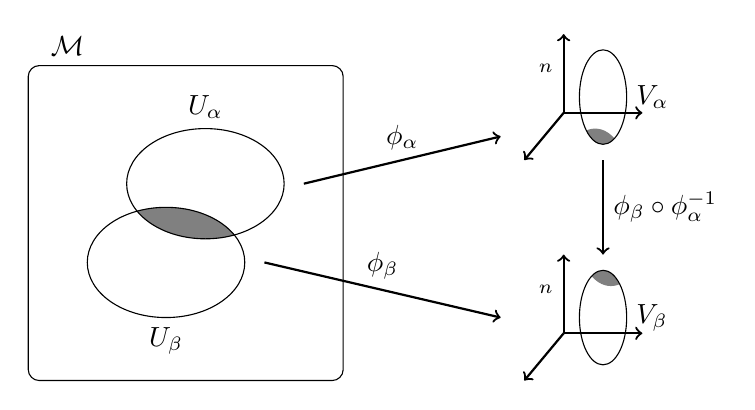
\begin{tikzpicture}
        \node[above] at (0.5,4) {\(\mathcal{M}\)};
        \draw[rounded corners] (0,0) rectangle (4,4);
        \begin{scope}
            \clip (1.75,1.5) ellipse (1 and 0.7);
            \fill[gray] (2.25,2.5) ellipse (1 and 0.7);
        \end{scope}
        \draw (1.75,1.5) ellipse (1 and 0.7);
        \draw (2.25,2.5) ellipse (1 and 0.7);
        \node[below] at (1.75,0.8) {\(U_\beta\)};
        \node[above] at (2.25,3.2) {\(U_\alpha\)};
        
        \begin{scope}[shift={(6.8,0.6)}]
            \draw[thick,->] (0,0) -- (1,0);
            \draw[thick,->] (0,0) -- (0,1);
            \draw[thick,->] (0,0) -- (-0.5,-0.6);
            \begin{scope}
                \clip (0.5,0.2) ellipse (0.3 and 0.6);
                \fill[gray] (0.6,1.2) ellipse (0.4 and 0.6);
            \end{scope}
            \draw (0.5,0.2) ellipse (0.3 and 0.6);
            \node[right] at (0.8,0.2) {\(V_\beta\)};
            \node[left] at (0,0.5) {\(\RR^n\)};
        \end{scope}
        
        \begin{scope}[shift={(6.8,3.4)}]
            \draw[thick,->] (0,0) -- (1,0);
            \draw[thick,->] (0,0) -- (0,1);
            \draw[thick,->] (0,0) -- (-0.5,-0.6);
            \begin{scope}
                \clip (0.5,0.2) ellipse (0.3 and 0.6);
                \fill[gray] (0.4,-0.8) ellipse (0.4 and 0.6);
            \end{scope}
            \draw (0.5,0.2) ellipse (0.3 and 0.6);
            \node[right] at (0.8,0.2) {\(V_\alpha\)};
            \node[left] at (0,0.5) {\(\RR^n\)};
        \end{scope}

        \draw[thick,->] (3.5,2.5) -- (6,3.1) node[midway,above] {\(\phi_\alpha\)};
        \draw[thick,->] (3,1.5) -- (6,0.8) node[midway,above] {\(\phi_\beta\)};
        \draw[thick,->] (7.3,2.8) -- (7.3,1.6) node[midway,right] {\(\phi_\beta\circ\phi_\alpha^{-1}\)};
    \end{tikzpicture}
\end{figure}
Informally, we can say that \(M\) is a topological space with some extra structure that allows us to introduce a differential calculus.

\begin{eg}
    The trivial manifold is \(\mathcal{M} = \RR^n\) with a single chart, for example the identity.
\end{eg}
Although it is not obvious, it is in fact usually possible to choose other differential structures on \(\RR^n\). For example, it has been shown that there are infinitely many \emph{exotic structures} on \(\RR^4\) (Donaldson 1984).
\begin{eg}
    The \(n\)-dimensional sphere \(S^n=\{\vb{r}\in\RR^{n+1}\st |\vb{r}|=1\}\subset \RR^{n+1}\) is an \(n\)-manifold. We choose open sets \(U = S^n \setminus N, \tilde{U} = S^n \setminus S\) where \(N = \{0,\dots,0,1\}\), \(S = \{0,\dots,0,-1\}\), and define charts as follows:
    \begin{figure}[H]
        \centering
        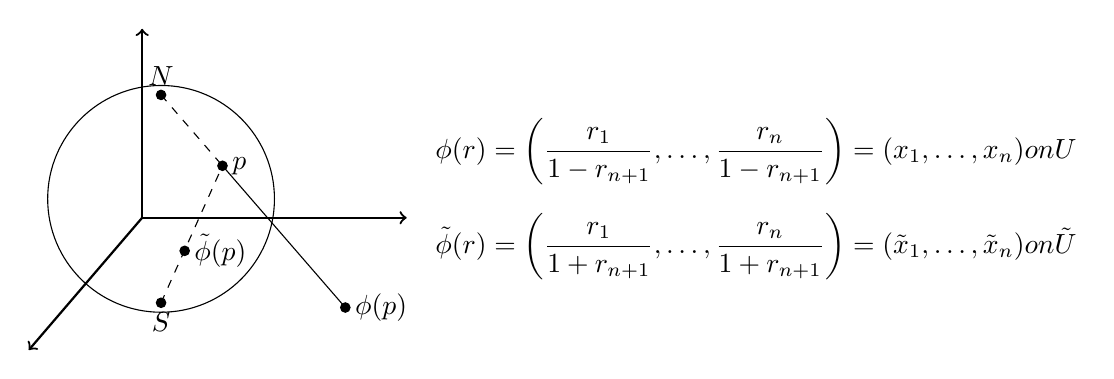
\begin{tikzpicture}[scale=1.2]
            \draw[thick,->] (0,0) -- (2.8,0);
            \draw[thick,->] (0,0) -- (0,2);
            \draw[thick,->] (0,0) -- (-1.2,-1.4);
            \draw (0.2,0.2) circle (1.2);
            
            \draw[dashed] (0.2,1.3) -- (0.85,0.55);
            \draw (0.85,0.55) -- (2.15,-0.95);
            \draw[fill] (2.15,-0.95) circle (0.05) node[right] {\(\phi(p)\)};

            \draw[dashed] (0.2,-0.9) -- (0.85,0.55);
            \draw[fill] (0.45,-0.35) circle (0.05) node[right] {\(\tilde\phi(p)\)};

            \draw[fill] (0.85,0.55) circle (0.05) node[right] {\(p\)};
            \draw[fill] (0.2,1.3) circle (0.05) node[above] {\(N\)};
            \draw[fill] (0.2,-0.9) circle (0.05) node[below] {\(S\)};

            \node[right] at (3,0.7) {\(\displaystyle
                \phi(\vb{r}) = \left( \frac{r_1}{1-r_{n+1}},\dots,\frac{r_n}{1-r_{n+1}} \right) = (x_1,\dots,x_n) \text{ on } U
            \)};
            \node[right] at (3,-0.3) {\(\displaystyle
                \tilde\phi(\vb{r}) = \left( \frac{r_1}{1+r_{n+1}},\dots,\frac{r_n}{1+r_{n+1}} \right) = (\tilde{x}_1,\dots,\tilde{x}_n) \text{ on } \tilde{U}
            \)};
        \end{tikzpicture}
    \end{figure}
    Note that:
    \begin{equation}
        x_1^2+\dots+x_n^2 = \frac{r_1^2+\dots+r_n^2}{(1-r_{n+1})^2} = \frac{1 - r_{n+1}^2}{(1-r_{n+1})^2} = \frac{1 + r_{n+1}}{1-r_{n+1}}
    \end{equation}
    So:
    \begin{equation}
        \tilde{x}_k = \frac{1-r_{n+1}}{1+r_{n+1}} x_k = \frac{x_k}{x_1^2+\dots+x_n^2}
    \end{equation}
    is smooth on \(U\cap \tilde{U}\).
\end{eg}

\begin{eg}
    Let \(f_1,\dots,f_k:\RR^N\rightarrow\RR\) and set \(M = \{\vb{r}\in\RR^N\st f_1 = \dots = f_k = 0\}\). Then \(M\) is a manifold if \(\rank\pdv{f^i}{x^a}\) is maximal, and is called a \emph{surface} in \(\RR^N\).
\end{eg}
In fact:
\begin{theorem}[Whitney]
    Any \(n\)-dimensional manifold \(\mathcal{M}\) can be obtained as a surface in \(\RR^N\), where \(N \le 2n+1\).
\end{theorem}
\begin{eg}
    Real projective space \(\mathbb{RP^n}\) is a manifold:
    \begin{equation}
        \mathbb{RP}^n = \frac{\RR^{n+1}\setminus{0}}{\sim} \qq{where} [X^1,\dots,X^{n+1}] \sim [cX^1,\dots,xC^{n+1}] \qq{for all} c \in \RR^* = \RR \setminus {0}
    \end{equation}
    We have \(n+1\) open sets \(U_\alpha = \{p\in\mathbb{RP}^n\st X^\alpha \ne 0\}\), and charts on each open set:
    \begin{equation}
        x_1 = \frac{X^1}{X^\alpha},\quad\dots\quad x_{\alpha-1} = \frac{X^{\alpha-1}}{X^\alpha},\quad x_{\alpha+1} = \frac{X^{\alpha+1}}{X^\alpha},\quad \dots\quad x_{n+1} = \frac{X^{n+1}}{X^\alpha}
    \end{equation}
\end{eg}

\section{Vector Fields}
\lecture{19/01/16}

Suppose we have two manifolds \(\mathcal{M},\tilde{\mathcal{M}}\) with dimensions \(n,\tilde{n}\), open sets \(U_\alpha,\tilde{U}_\beta\) and charts \(\phi_\alpha,\phi_\beta\) respectively, and let \(f\) be a map from \(\mathcal{M}\) to \(\tilde{\mathcal{M}}\).

\begin{defn}
    \(f\) is \emph{smooth} if \(\tilde{\phi}_\beta\circ f\circ\phi_\alpha^{-1}:\RR^n\rightarrow\RR^{\tilde{n}}\) is smooth for all \(\alpha, \beta\).
\end{defn}

\begin{defn}
    If \(\tilde{\mathcal{M}}=\RR\), then \(f:\mathcal{M}\rightarrow\RR\) is a \emph{function}.
\end{defn}

\begin{defn}
    If \(\mathcal{M} = \RR\), then \(f:\RR\rightarrow\tilde{\mathcal{M}}\) is a \emph{curve}.
\end{defn}

Suppose we have a curve \(\gamma:\RR\rightarrow\mathcal{M}\) such that \(\gamma(0) = p \in \mathcal{M}\). Let \(U\) be an open neighbourhood of \(p\), \(U\simeq\RR^n\) and choose coordinates \(x^a\), \(a = 1,\dots,n\) on \(U\).

\begin{defn}
    The \emph{tangent vector} to \(\gamma\) at \(p\) is defined as:
    \begin{equation}
        V|_p = \left.\dv{\gamma(\epsilon)}{\epsilon}\right|_{\epsilon=0}\in T_p\mathcal{M}
    \end{equation}
    where \(T_p\mathcal{M}\) is the \emph{tangent space} at \(p\), defined as the set of all tangent vectors to all curves at \(p\).
    \begin{figure}[H]
        \centering
        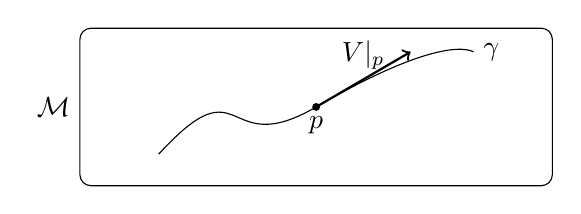
\begin{tikzpicture}
            \draw[rounded corners] (0,0) rectangle (6,2);
            \node[left] at (0,1) {\(\mathcal{M}\)};
            \draw (1,0.4) .. controls (2.1,1.6) and (1.8,0.3) .. (3,1)
                          .. controls (4.2,1.7) and (4.8,1.8) .. (5,1.7)
                          node[right] {\(\gamma\)};
            \fill (3,1) circle (0.05) node[below] {\(p\)};
            \draw[->, thick] (3,1) -- (4.2,1.7) node[midway,above] {\(V|_p\)};
        \end{tikzpicture}
    \end{figure}
\end{defn}

\begin{defn}
    The \emph{tangent bundle} is given by:
    \begin{equation}
        T\mathcal{M} = \bigcup_{\mathclap{p\in\mathcal{M}}} T_p\mathcal{M}
    \end{equation}
\end{defn}

A vector field assigns a tangent vector to each point \(p\in\mathcal{M}\). Let \(f:\mathcal{M}\rightarrow\RR\). The rate of change of \(f\) along \(\gamma\) is given by:
\begin{align}
    \dv{\epsilon}f(x^a(\epsilon))|_{\epsilon=0} &= \sum_{a=1}^n \dot{x}^a(\epsilon)\left.\pdv{f}{x^a}\right|_{\epsilon=0}\\
    &= \underbrace{\sum_{a=1}^nV^a(x)\left.\pdv{x^a}\right|_p}_{=V} f
\end{align}
\(V\) is a vector field. \(V^a(x)\) are the components of \(V\) in the basis \(\left\{\pdv{x^1},\dots,\pdv{x^n}\right\}\) at \(p\). 

We have gone from a curve to a vector field. We can also go the other way:
\begin{defn}
    An \emph{integral curve} or \emph{flow} \(\gamma(\epsilon)\) of a vector field \(V\) is defined by:
    \begin{equation}
        \dot{\gamma}(\epsilon) = V|_{\gamma(\epsilon)}
        \qq{or, equivalently}
        \dv{\epsilon}x^a(\epsilon) = V^a(x(\epsilon))
    \end{equation}
\end{defn}
We have:
\begin{equation}
    x^a(\epsilon,x^a(0)) = x^a(0) + \epsilon V^a(x(0)) + O(\epsilon^2)
\end{equation}
We say that the vector field \(V\) \emph{generates} the flow.
\begin{defn}
    An \emph{invariant} of a vector field \(V\) is a function that is constant along the flow of \(V\):
    \begin{equation}
        f(x^a(0)) = f(x^a(\epsilon)) \Forall \epsilon
        \qq{or, equivalently}
        V(f) = 0
    \end{equation}
\end{defn}
\begin{eg}
    Let \(\mathcal{M}=\RR^2\), \(x^a = (x,y)\), and \(V = x\pdv{x}+\pdv{y}\). The integral curves of \(V\) are given by \(\dot{x}=x\), \(\dot{y}=1\), and we can solve this to obtain \((x(\epsilon),y(\epsilon)) = (x(0)e^\epsilon,y(0)+\epsilon)\).
    \begin{figure}[H]
        \centering
        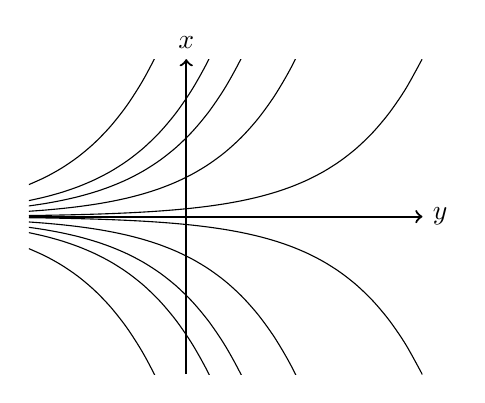
\begin{tikzpicture}
            \draw[thick,->] (-2,0) -- (3,0) node[right] {\(y\)};
            \draw[thick,->] (0,-2) -- (0,2) node[above] {\(x\)};
            \clip (-2,-2) rectangle (3,2);
            \draw[domain=-2:3,smooth,variable=\x] plot ({\x},{3*exp(\x)});
            \draw[domain=-2:3,smooth,variable=\x] plot ({\x},{1.5*exp(\x)});
            \draw[domain=-2:3,smooth,variable=\x] plot ({\x},{exp(\x)});
            \draw[domain=-2:3,smooth,variable=\x] plot ({\x},{0.5*exp(\x)});
            \draw[domain=-2:3,smooth,variable=\x] plot ({\x},{0.1*exp(\x)});
            \draw[domain=-2:3,smooth,variable=\x] plot ({\x},{-0.1*exp(\x)});
            \draw[domain=-2:3,smooth,variable=\x] plot ({\x},{-0.5*exp(\x)});
            \draw[domain=-2:3,smooth,variable=\x] plot ({\x},{-exp(\x)});
            \draw[domain=-2:3,smooth,variable=\x] plot ({\x},{-1.5*exp(\x)});
            \draw[domain=-2:3,smooth,variable=\x] plot ({\x},{-3*exp(\x)});
        \end{tikzpicture}
    \end{figure}
    Note that on these curves \(xe^{-y}\) is constant, so this is an invariant of \(V\).
\end{eg}
\begin{eg}
    Consider the 1-parameter group of rotations on \(\RR^2\). Under these rotations, \((x_0,y_0)\) transforms to the point \((x(\epsilon),y(\epsilon)) = (x_0\cos\epsilon-y_0\sin\epsilon,x_0\sin\epsilon+y_0\cos\epsilon)\). The vector field that generates these curves is given by:
    \begin{align}
        V &= \left( \dv{y(\epsilon)}{\epsilon}\pdv{y} + \dv{x(\epsilon)}{\epsilon}\pdv{\epsilon} \right)\\
        &= x\pdv{y} - y\pdv{x}
    \end{align}
    The distance to the origin is an invariant of \(V\):
    \begin{equation}
        V(x^2+y^2) = -2xy + 2xy = 0
    \end{equation}
\end{eg}
\begin{defn}
    A \emph{Lie bracket} of two vector fields \(V\) and \(W\) is a vector field \([V,W]\) defined by its action on functions as:
    \begin{equation}
        [V,W](f) = V(W(f))-W(V(f))
    \end{equation}
\end{defn}
The Lie bracket has some important properties:
\begin{description}
    \item[Antisymmetry]: \([V,W] = -[W,V]\)
    \item[Jacobi identity]: \([U,[V,W]] + [V,[W,U]] + [W,[U,V]] = 0\)
\end{description}
\begin{eg}
    If \(V = x\pdv{x}+\pdv{y}\) and \(W = \pdv{x}\), then \([V,W] = -\pdv{x} = -W\).
\end{eg}
\begin{defn}
    A \emph{Lie algebra} is a vector space \(\mathfrak{g}\) equipped with an antisymmetric bilinear operation \([\;,\;]:\mathfrak{g}\times\mathfrak{g}\rightarrow\mathfrak{g}\) that satisfies the Jacobi identity.
\end{defn}
If \(\mathfrak{g}\) is finite-dimensional and \(V_\alpha\), \(\alpha = 1,\dots,\dim\mathfrak{g}\) span \(\mathfrak{g}\), then \(\mathfrak{g}\) is determined by its structure constants \(f_{\alpha\beta}^\gamma\), defined as follows:
\begin{equation}
    [V_\alpha,V_\beta] = \sum_\gamma f_{\alpha\beta}^\gamma V_\gamma
\end{equation}
\begin{eg}
    There are only two 2D Lie algebras (up to isomorphism), each determined by the bracket of two basis elements:
    \begin{equation}
        [V,W] = 0 \qq{or} [V,W] = -W
    \end{equation}
\end{eg}
\begin{eg}
    \(gl(n,\RR)\) (the set of all \(n\times n\) real matrices) is a Lie algebra when equipped with the matrix commutator as a bracket. Its dimension is \(n^2\).
\end{eg}
\begin{eg}
    Vector fields on a manifold \(\mathcal{M}\) form an infinite dimensional Lie algebra. Consider for example \(\mathfrak{g} = \operatorname{diff}(S^1)\) or \(\operatorname{diff}(\RR)\), by which we mean the set of all vector fields on the manifold. We have the following basis of \(\mathfrak{g}\):
    \begin{equation}
        V_a = - x^{\alpha+1}\pdv{x} \qq{where} \alpha\in\ZZ
    \end{equation}
    With this basis, the Lie bracket gives:
    \begin{equation}
        [V_\alpha,V_\beta] = (\alpha-\beta)V_{\alpha+\beta}
    \end{equation}
\end{eg}
\end{document}
